\chapter{Related Works}
\label{chapter:related}

%\minitoc
\chapterwithfigures{\nameref*{chapter:related}}
%\chapterwithtables{\nameref*{chapter:introduction}}

\ifthenelse{\boolean{skipRelated}}{\endinput}{}

\section{Continual Learning}

What is continual, iid, forgetting

evaluation, multi-head, single-head

class incremental, domain incremental, new class and new domain incremental. \cite{lomonaco2017core50}

\begin{figure}[tb]
    \begin{center}
        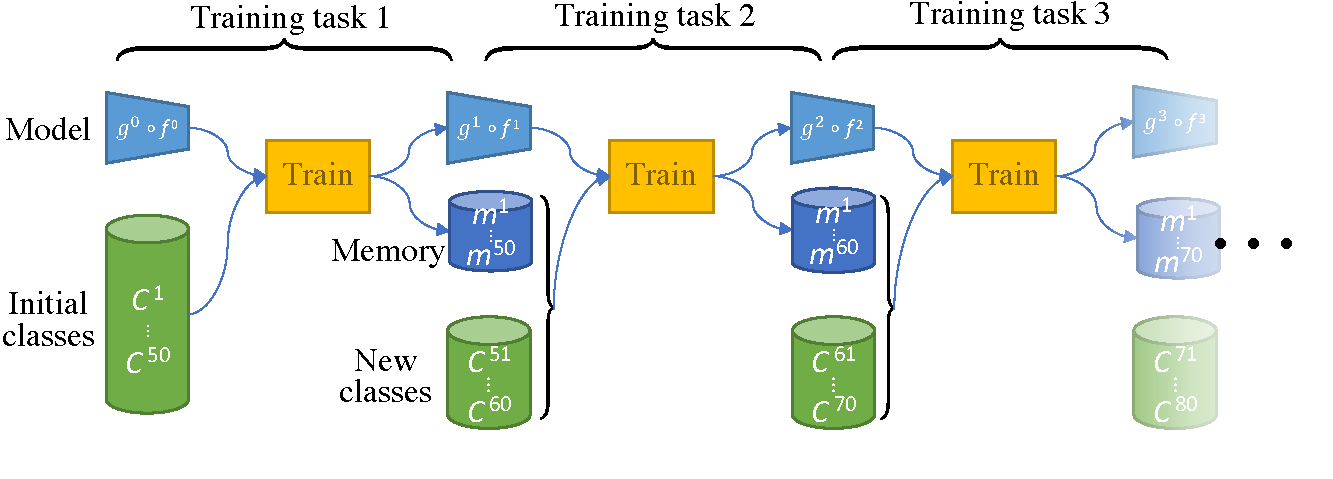
\includegraphics[width=0.8\linewidth]{images/podnet/protocol}
    \end{center}
    \caption{\textbf{Training protocol for incremental learning}. At each training task we learn a
        new set of classes, and the model must retain knowledge about \textit{all} classes. The
        model is allowed a \textit{limited} memory of samples of old classes.}
    \label{fig:protocol}
\end{figure}


\section{Rehearsal}

\citep{lesort2019regulshortcomings} showed that

\section{Regularization-based Approaches}

\subsection{Weight-based}

\subsection{Gradient-Based}

\subsection{Output-based}

\section{Dynamic Strategies}



\section{Optimization}

